\documentclass[12pt]{article}
 
\usepackage[utf8]{inputenc}
\usepackage[T1]{fontenc}
\usepackage{lmodern}
\usepackage[ngerman]{babel}
\usepackage{geometry}
\geometry{a4paper}

\usepackage{amsmath}
\usepackage[urlcolor=blue]{hyperref}
\usepackage{graphicx}
\usepackage{setspace}
\onehalfspacing

 
\title{Praktikumsbericht}
\author{Josef Schulz}
\date{20. Februar 2014}
\begin{document}
 
\maketitle

\newpage

\tableofcontents

\newpage

\section{Vorbetrachtung}

\subsection{Begebenheiten}

Die Leidenschaft zur Informatik habe ich bei meinen ersten Programmierversuchen in der Schulzeit entwickelt.
In den Folgenden Jahren begann ich meine Kenntnisse zu vertiefen und meine Fähigkeiten, im Theoretischen
und im Praktischen weiter zu verbessern. Das Studium der Informatik an der TU-Dresden bietet die Möglichtkeit,
ein 20-Wöchiges Praktikum zu absolvieren oder ein Semester im Ausland Studieren zu können.

Einige meiner Professoren bemängelten während der Vorlesungen die Üngenügende Praktische Erfahrungen von
Absolventen. Zu dem zeigte sich mir, in den Vergangenen Semestern wie viel Zeit sich durch ausreichende Übung,
bei der Realisierung von Algorithmen einsparen lässt. Im Theoretischen scheint die eigentliche Programmierung
oft als Trivialer Faktor. In der Praxis zeigt sich, das diese Arbeit oft langwieriger gestalltet als zuvor
gedacht. So bleibt nach Aussage eines Professors, oft keine Zeit mit Parametern zu experimentieren.
Ein Praktikum motiviert zum Sammeln von Praktischen Erfahrungen, veranlasst ein Umdenken, da man neue Ideen und
Technologien kennen lernt, was nur zum Vorteil des Praktikanten sein kann.

Eine gute Möglichkeit für Praktikas bieten insbesondere kleinere Unternehmen, da in diesen die Mitarbeiter
viele Aufgaben auf sehr wenige Verteilen müssen. Ein Praktikant wird dadurch stark in den Entwicklungsprozess
mit einbezogen. Weiterhin zeigt sich dem Praktikant der Stand seiner eigenen Entwicklung als Informatiker.

\subsection{Nützlichkeiten}

Das Informatikstudium an der TU-Dresden verlangt den Studenten eine Gruppenarbeit während des dritten Semesters
ab. Für nicht wenige ist dieses, das erste Projekt in dem sie mit anderen zusammen an einem Gemeinsamen Ziel
arbeiten müssen. Neben der Kommunikation, verlangt die Menge an Quelltext-Zeilen eine gute Organisation und
kommunikation. 

Die Arbeit aus dem dritten Semster umfasst in etwa 8000 Zeilen Quelltext. In Realen Programmen, steigt die
Anzahl von Zeilen und von verwendeten Technologien stark an. Diese Erfahrungen sehe ich als große Bereicherung.

Bevor ich die Firma und meinen Aufgabenbereich erläutere, möchte ich einen kurzen abriss meiner Vertiefungen
aus den höhren Semstern meines Studiums geben. Mein Hauptaugenmerk liegt im Bereich der Grafikprogrammierung,
der Bildverarbeitung und insbesondere im Gebiet des Maschinellen Lernens. Mit Softwaretechnologie habe ich mich
zu diesem Zeitpunkt nur im Rahmen meines Grundstudiums beschäftigt. Das Gebiet der Webentwicklung, habe ich nur
am Rande durch das Softwaretechnologiepraktikum im dritten Semester kennen gelernt, das bereits mehr als ein
Jahr zurück liegt. 

\subsection{Formalitäten}

Das für das Praktikum beanschlagte Zeitrum beträgt 20 Wochen, diese habe ich im Zeitraum vom 1. September 2013
bis zum 31. Januar 2014, in der \href{https://alaun.de/home/}{Alaun GmbH} absolviert.

\section{Alaun GmbH}

\subsection{Impressum}

\begin{minipage}{\linewidth}

alaun GmbH \\
Hoyerswerdaer Straße 20 \\
01099 Dresden \\

Tel (0351) 563406-0  \\
Fax (0351) 563406-29 \\

mail@alaun.de 

\end{minipage}

\subsection{Übersicht}

Bei der \href{https://alaun.de/home/}{Alaun GmbH} handelt es sich um ein Unternehmen mit Sitz in Dresden.
Die \href{https://alaun.de/home/}{Alaun GmbH} beschäftigt 11 Mitarbeiter, die auf zwei Hauptprojekte verteilt
sind. Das erste, Business ByDesign soll hier nur der Vollständigkeitshalber erwähnt werden, 
da ich an diesem Projekt nicht beteiligt war. Das zweite trägt Firmen Intern den Titel \textit{Eine neue Welt},
es ist ehr ein Arbeitsbegriff für zwei Content Management Systeme, im Folgenden mit CMS abgekürzt deren Inhalte
ich im entsprechenden Unterpunkt erläutern werde.

\subsection{Business ByDesign}

Unter dem Namen Business ByDesign werden Anwendungen und Komplettlösungen anderer Unternehmen für den
Endkunden angepasst. So auch eine SAP Software die bei einer in Dresden ansässigen Brauerrei zum Einsatz kommt.

\subsection{Eine neue Welt}

Im Jahr 2001 began der Verkauf des CMS-tools Elexir an die Sparkassen Deutschlandweit. Mit diesem Tool werden
die Internetauftritte der einzelnen Institute gestalltet. Besonders hervor zu heben ist die Größenordung und
die Anzahl der zu verwaltenden Projekte. Jedes Institut gestalltet im Prinzip unabhängig von den anderen seine Onlinepräsenz.
Gänzlich voneinander zu trennen sind diese auch nicht, da Werbung, Kundeninformationen und Designs in
Regionen basierten Hierarchien vorgegeben und geteilt werden.

Nach 13 Jahren Laufzeit hat die \href{https://alaun.de/home/}{Alaun GmbH} mit einer Neuauflage des Projektes begonnen.
Mit einem Sprachbasierten Ansatz wird Problemen begegnet, die durch Verteilte Entwicklung in dieser Größenordnung
entstehen. Namen und Ids werden Automatisch generiert und vor dem Benutzer verborgen. 
Die Entwickelte Sprache, trägt den Namen Cauldron und wird durch ein Java-Backend realisiert.
Cauldron ist eine XML-Basierte Sprache und dient zur Entwicklung von Internetseiten.
Im Gegensatz zu HTML, gibt es eine Vererbungshierachie. Durch diese wird Redundanz beim Programmieren vermieden.
Neben den sogenannenten \textit{namespaces} gibt es noch \textit{Module} und \textit{Fragmente} durch die sich,
Programmkomplexe kapseln und überlagern können. 


\section{Der Verlauf}

\subsection{Der erste Arbeitstag}

Am 2. September 2013 um 0900 begann für mich die Zeit in der \href{https://alaun.de/home/}{Alaun GmbH}.
Zu beginn lernte ich die Firma kennen und die bereits oben erwähnten Projekte wurden mir erläutert.
Da die \textit{neue Welt} zu diesem Zeitpunkt besonderen Entwicklungsaufwand bedurfte entschied ich mich
an diesem Projekt aktiv teil zu nehmen.

Um mich mit der Thematik vertraut zu machen, lass ich das Pflichtenheft und sämtliche Dokumente, die die Firma
zu diesem Projekt verfasst hat. 

\subsection{Entwicklungsumgebung und Technologien}

Nach der Grundlegensten Einarbeitung begann ich die Entwicklungsumgebung einzurichten und mich in Technologien
wie zum Beispiel Maven und OSGI einzuarbeiten. Die \href{https://alaun.de/home/}{Alaun GmbH} hat für die Korrektur
des Cauldron-Quelltextes ein eigenes Plugin bereitgestellt, durch welches die Entwicklung eigener Cauldronbasierter
Projekte erleichtert wird. Interprettiert wird der Cauldron-Quelltext durch ein Java-Servlet. 
Da für die Einrichtung der Entwicklungsumgebung noch keine Dokumente existierten, dokumentierte ich meine Schritte
um nachfolgenden Programmieren einen Schnelleren Einstieg in das Projekt zu ermöglichen.

Meine Kenntnisse auf dem Gebiet der Web-Programmierung ließen noch zu wünschen übrig, deshalb begann ich mit der Entwicklung
eines primitiven Funktionsplotters. Ziel der Übung war es mich mit Cauldron erst einmal vertraut zu machen.
Ich bekam Unterstützung von einem Versierten Kollegen, der mir nicht nur Programmiertechnische Aspekte der Web-Entwicklung näherbringen konnte.
Farben und Aufteilungen waren ebenfalls Bestandteil meines Trainings. 
Zum Zeichnen der Funktionen diente ein Canvas Element und Javascript.
Nach der Fertigstellung des Funktions-Plotters für einen Normalen Browser, konnte ich mit den Methoden von Cauldron
binnen kürzester Zeit eine Mobile Version der Seite fertig stellen.
Hier zeigten sich die Vorzüge von Komponenten und Vererbungen, mit deren hilfe sich die Anzahl an Quelltextzeilen gering gehalten
werden konnte.

\subsection{Entwicklung von Komponenten}

Entwickelt man ein CMS-System, sind einfache Komponenten wie Textfeldern und Bezeichnern, welche von HTML bereitgestellt werden
nur ein Anfang. Im Folgenden begann ich bei der Entwicklung der Komponenten zu helfen. Als Beispiel dient eine Einfache Textbox
mit Bezeichner. Eine Solche Komponente bringt mehrere Variablen mit sich. Damit ist zum einen der Inhalt des Bezeichners und der
Voreingestellte Inhalt der Textbox gemeint, zum anderen werden aber auch die möglichkeiten zum Gestalten und Platzieren vorgegeben.
Auf diese Weise können sehr komplexe Komponenten entstehen, so lässt sich eine breite Pallete an Bankformularen konzipieren.

Cauldron bietet aber noch viel mehr, als Designs und Formulare. Der Workflow ist eine Backendbassierte realisierung eines 
Mealyautomaten. Durch den Einstatz von Workflows lassen sich Funktionale Komponenten konstruieren die sich im späteren Editor
mit der Maus schnell auf eine Seite ziehen lassen.

Eine Komponente ist eine Art Kontainer, mit der Möglichkeit Parameter zu übergeben und den Einsatz möglichst Variable zu gestallten.
Komponenten können von anderen Komponenten erben und haben eine gewisse Ähnlichkeit mit Klassen. Daher eignet sich UML sehr gut zur
Modelierung von von Komponentenstrukturen.

\begin{figure}[h]
	\centering
	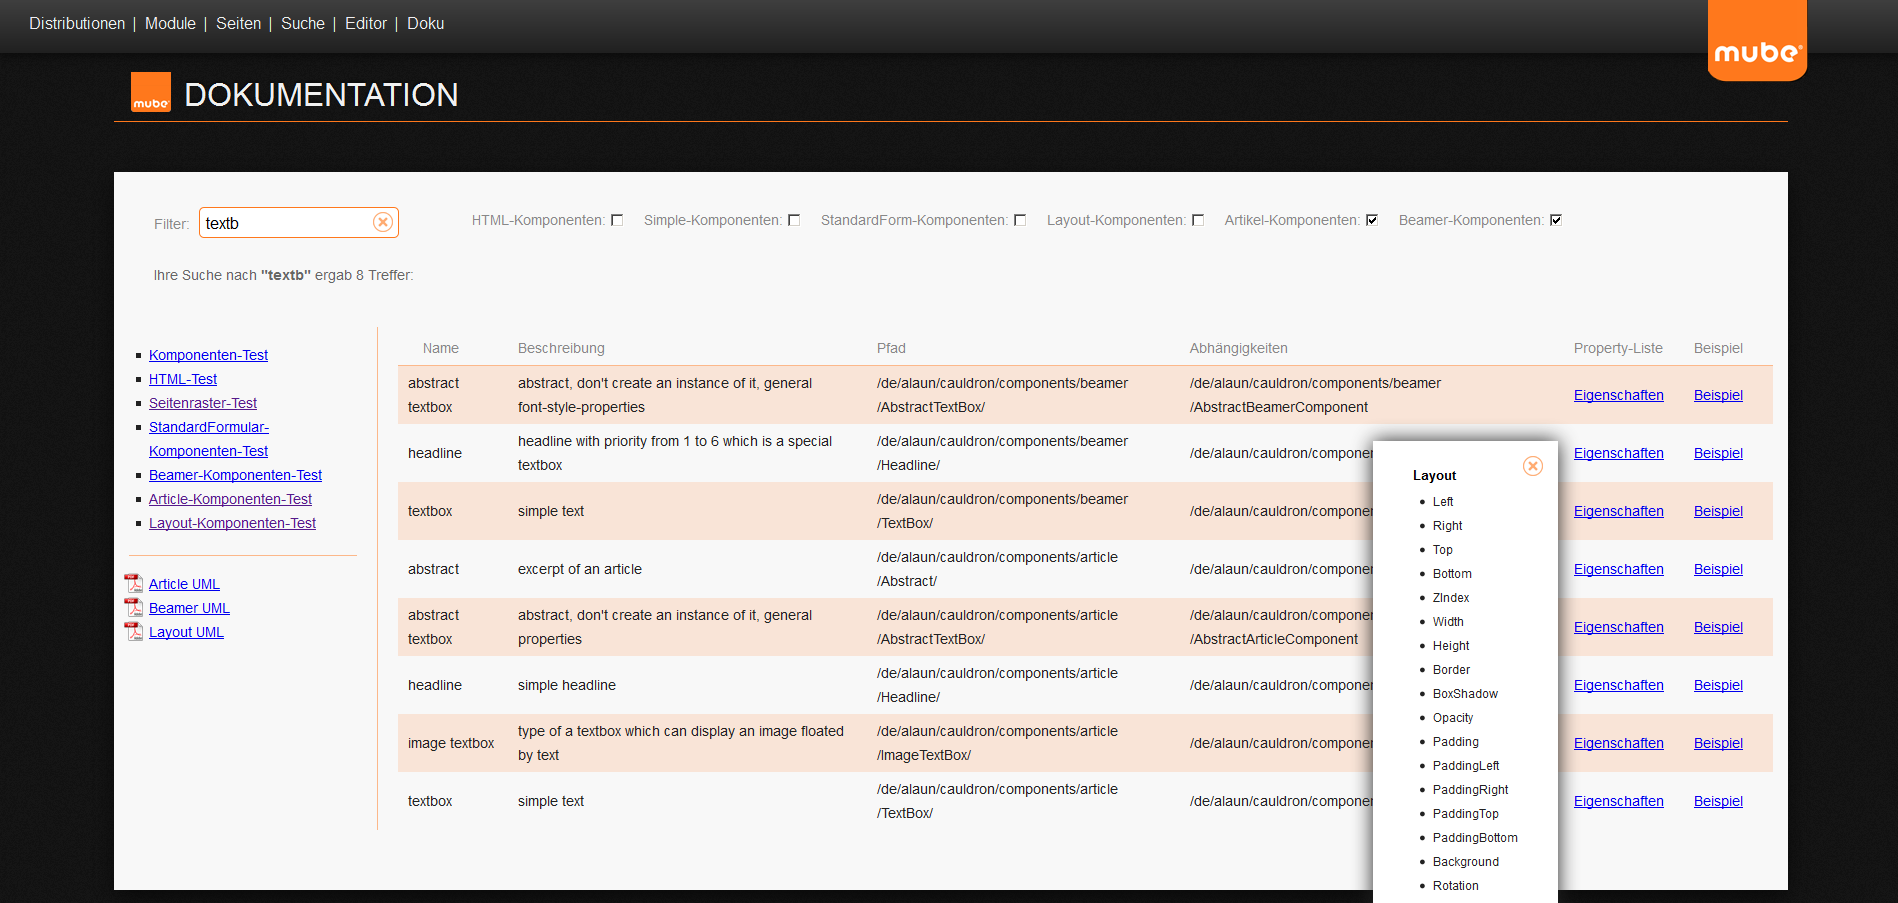
\includegraphics[width=1.0\textwidth]{DokuPage.png}
	\caption{Komponenten Dokumentation}
	\label{fig:DokuPage}
\end{figure}

Neben der Entwicklung der Komponenten, haben wir eine Dokumentation dieser erstellt. Im Verlauf dieser Entwicklung haben wir
den Prozess der Dokumentierung vereinfacht. Um nicht jedes mal an mehreren Stellen bei Änderungen die Einträge bearbeiten zu müssen,
führten wir Tags ein. Mögliche Variablenbelegungen wurden Automatisch aus den Komponenten gezogen. Ein Ausschnit der Dokumentation
wird in der Abbildung \ref{fig:DokuPage} dargeboten.

\subsection{Seitenlayouts}

\begin{figure}[h]
	\centering
	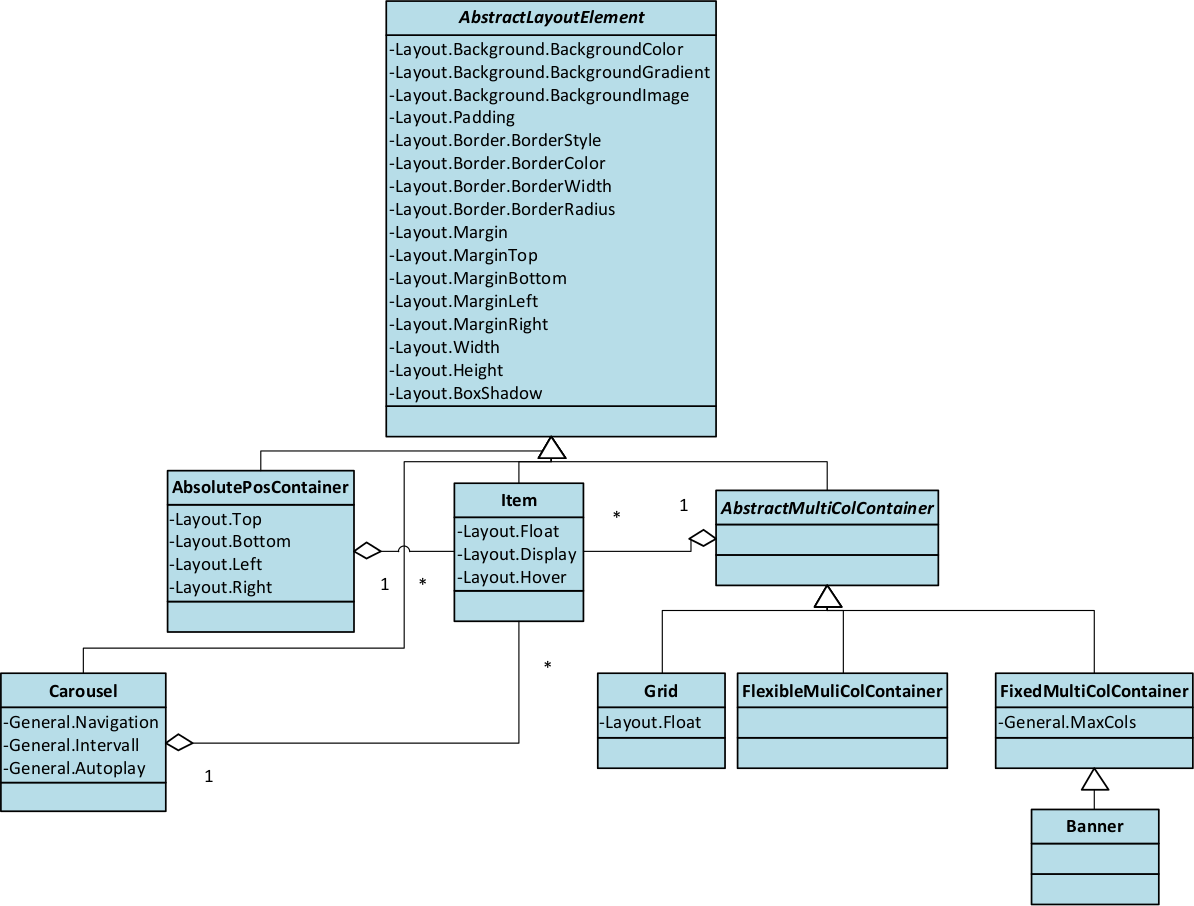
\includegraphics[width=1.0\textwidth]{Layout.png}
	\caption{Layoutkomponenten UML-Diagram}
	\label{fig:Layout}
\end{figure}

Ein weiteres Aufgabenfeld bestand in der Entwicklung von Komponenten für Standartisierte Seitenformen, wie den Artikel und
eine Präsentationskomponente. In beiden Fällen haben wir bestehende Programme studiert und daraus eine Komponenten-Strukuren
mit UML-Diagrammen abgeleitet und ergänzt. Die Abbildung \ref{fig:Layout} zeigt die Komponenten Struktur für unsere Layout-Kontainer mit deren
hilfe sich Inhalte automatisch anordnen lassen.

\subsubsection{Präsentations-Komponenten}

\begin{figure}[h]
	\centering
	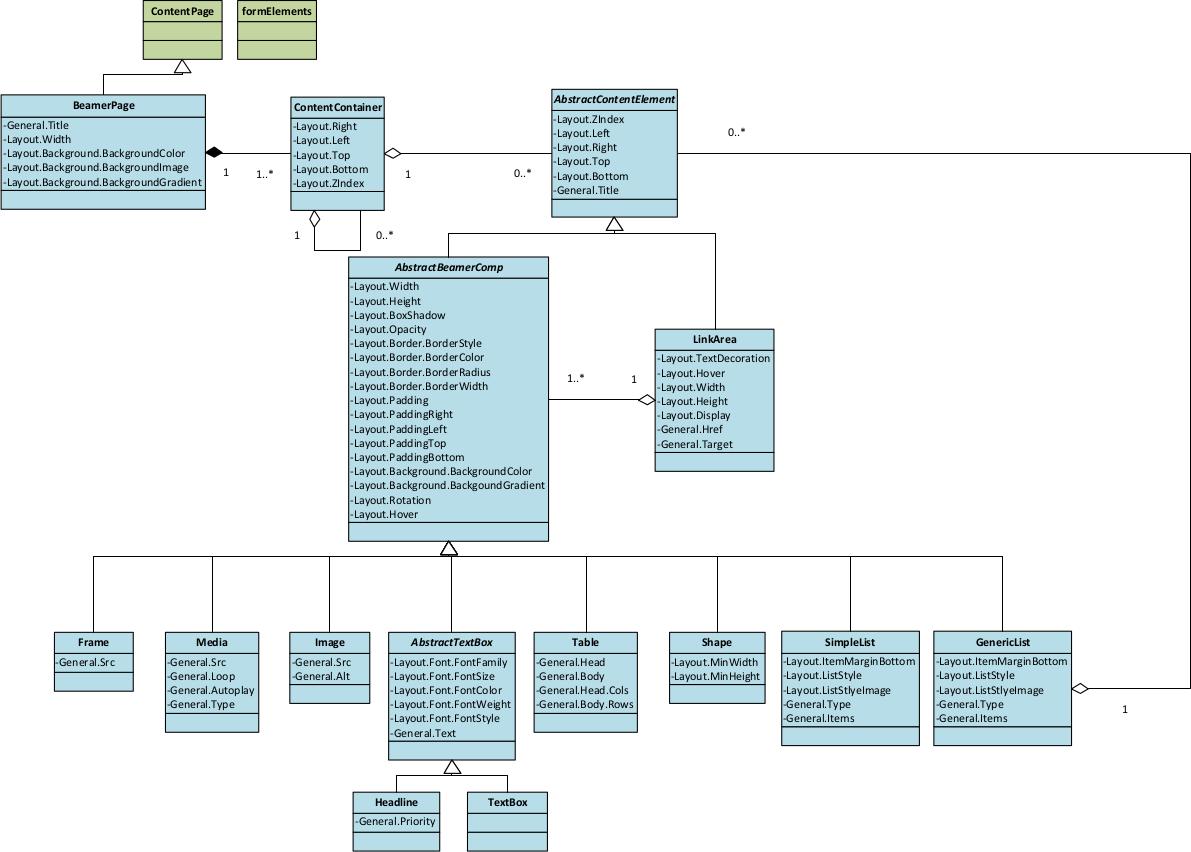
\includegraphics[width=1.0\textwidth]{Beamer.png}
	\caption{Präsentationskomponenten UML-Diagram}
	\label{fig:Beamer}
\end{figure}

Die Präsentationsseite besteht aus mindestens einen Kontainer für Inhalt, diese können jeweils wieder aus Kontainern oder aus Elementen bestehen.
Es gibt eine vielzahl von Elementen die sich innerhalb eines Kontainers absolute possitionieren lassen. Die Abbildung \ref{fig:Beamer} zeigt
das UML-Diagramm das die Komponenten Struktur unserer Präsentations-Komponenten wiederspiegelt. 

Um einen kurzen Einblick in die Funktionsweise unsere Präsentationskomponenten zu geben möchte ich auf die \textit{LinkArea} etwas genauer eingehen. 
Die Grundlegenden Elemente die in einem Kontainer plaziert werden können, werden als \textit{AbstractContentElement} bezeichnet. Von diesem leitet
sich auf der einen Seite die \textit{AbstsractBeamerComp} und auf der anderen Seite die \textit{LinkArea} ab. Letztere besteht ebenfalls wieder
aus Elementen des Typs \textit{AbstsractBeamerComp}. In einer \textit{LinkArea} enthaltene Elemente dienen zur Gestaltung des Links. Farben und Formen
können überschrieben werden, wodurch sich zum Beispiel Farben beim sogenannten Hovereffekt verändern lassen.

\subsubsection{Artikel-Komponenten}

\begin{figure}[h]
	\centering
	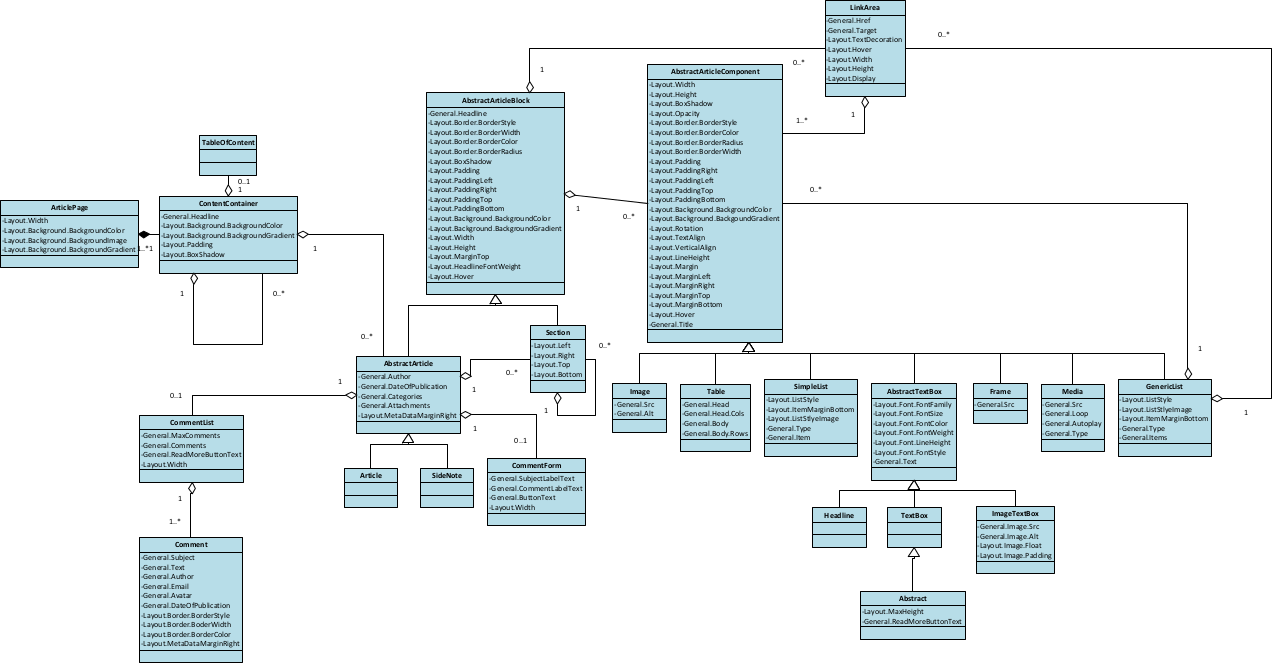
\includegraphics[width=1.0\textwidth]{Artikel.png}
	\caption{Artikelkomponenten UML-Diagram}
	\label{fig:Artikel}
\end{figure}

Die Artikel Komponenten bilden einen weiteren Seitentyp der aus einer vielzahl von bestehenden Programmen
bekannt sein dürfte. In der Abbildung \ref{fig:Artikel} das entsprechende UML-Diagram dargeboten.
Der Prinzipelle Aufbau erinnert an die Präsentationskomponenten, er unterscheidet sich aber hinsichtlich
der Positionierungen und Unterteilungen. Ist eine Präsentation auf eine bestimmte Seitengröße festgelegt, ist diese bei der Artikelseite
nicht vorgegeben. Artikel können beliebig lange Seitenverläufe Formen sich aber auch in kleinere Seiteneinheiten unterteilen lassen.
Direkt integriert ist in Anlehnung an diverese Blogs eine Komentarliste mit dem entsprechenden Formular zum hinterlassen
von Komentaren entstanden.

\subsection{Intermezzo}

Nach der Entwicklung dieser Komponentenstrukturen hatte ich die nötige Zeit um mich mit WebGl zu beschäftigen. Durch WebGL ist es Möglich
komplexe Szenen direkt im Browser darzustellen. Zu Gestalltung der Seitenkomponenten, welche nicht durch WebGL gerendert wurden, wie \textit{Buttons}
und \textit{Checkboxen} benutze ich HTML und CSS ohne Cauldron. Dabei zeigten sich die Vorzüge Cauldron besonders deutlich.
Der Unterschied war um so gravierender je mehr Identische Objekte auf einer Seite benötigt wurden. Diese Erfahrung zerstreute den Rest Skepsis
den ich gegenüber des Cauldronprojektes bis zu diesem Zeitpunkt hatte. Durch die Entwicklung mit WebGl lernte ich einiges über Javascript,
insbesondere was die Effizens verschiedener Implementierungen angeht. Der Einsatz von WebGl könnte ebenso für besondere Darstellungsvarianten
in das CMS integriert werden. Als bespiel könnte die Animation eines Sparkassensymbols dienen. Im gegensatz zu einfachen Gifs wäre es Interaktiv
und bietet nahezu unbegrenzte Möglichkeiten. Der Einsatz auf Mobilen geräten, ist aber auf Grund der benötigten Rechenleistung ehr ein
Zukunftstraum. Eine Interesannte Möglichkeit würde sich durch das Rendern von HTML in Texturen ergeben. Man wäre in der Lage Inhalte flexibel in
einem Dreidimensionalen Raum zu bewegen. Eingabegeräte könnten ebenfalls in den 3D-Raum abgebildet werden.

\subsection{Altes wird auch neu}

Neben dem bisher behandelten neubau eines CMS-Tools, pflegt die \href{https://alaun.de/home/}{Alaun GmbH} den Vorgänger mit dem Namen Elexir.
Updates und neuerungen werden nach wie vor für das alte Eisen produziert. Die Struktur von Elexir erlaubt es ebenfalls mit einer XML-Basierten
Sprache anzupassen vorzunehmen. Die \href{https://alaun.de/home/}{Alaun GmbH} stellt externen Firmen Werkzeuge zur Entwicklung für derartige
Erweiterungen bereit. Um diese Erweiterungen in Elexir einspielen zu können, haben wir einen Addon Manager entwickelt. Dieses Tool besteht
ebenfalls aus eine Reihe von Scripts und ermöglich die Anbindung an einen Händler für diese Addons.

Bisher wurden Erweiterungen und Neuerungen zu bestimmten Releasezeitpunkten in Form von Gepackten Archiven händisch von den Admininstratoren
in Elexir eingespielt. Mit der Lieferung des Addon-Managers ist diese Vorgehensweise nur noch ein letzes mal nötig.

Die Addons von Externen Firmen werden als Verschlüsselte Version mittels Git von den Alaunservern angezogen. Bevor diese dann als Neuerscheinung
oder als Update im Store erscheinen, werden die Addons von einem Programm auf vollständigkeit überprüft und entsprechend Freigeschalten oder
zurückgehalten. 

\begin{figure}[h]
	\centering
	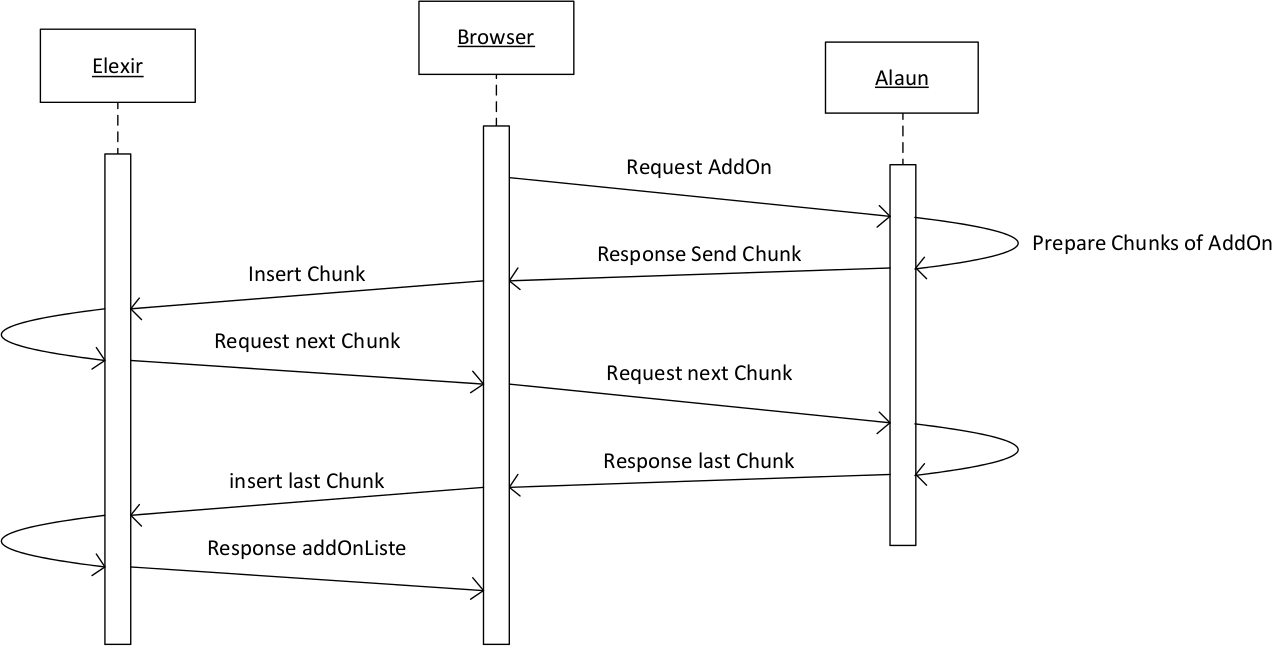
\includegraphics[width=1.0\textwidth]{Manager.png}
	\caption{Download Squenzdiagram}
	\label{fig:Manager}
\end{figure}


Der AddonManager lösst die Kommunikation zwischen dem entsprechenden Elexirclienten und den Alauen-Servern. Ein Elexirclient kann nicht direkt
mit den Alaunservern kommunizieren, da beide über eine \textit{HTTPS} Verbindung laufen. Als Schnittstelle dient der Browser des Elexirnutzers.
Die Kommunikation ist Beispielhaft in Abbildung \ref{fig:Manager} dargestellt. 

Beim Zugriff auf den AddonManager wird ein \textit{JSONP-Request} ausgeführt, mit dessen hilfe wird eine Liste mit AddonId und Version an die
Alaunserver gesendet. Der nächste Schritt besteht aus einem Aktuallitätscheck. Die Alaunserver vergleichen die Addonversionen und setzt gegebenenfalls
ein Flag. Die Liste an updatebaren Addons wird dem Browser jetzt als Parameter der Responsefunktion übergeben.

Im Folgenden wird dem Nutzer eine Liste mit seinen Addons angezeigt. Wurde das Flag für \textit{update} gesetzt, dann wird ein Button herausgerendert
über welchen das spezifische Addon aktuallisiert werden kann. Weiterhin besteht die Möglichkeit alle Addons in einem Schritt zu aktuallisiern.
Neue Addons können über den Addonstore erworben werden. Dazu wird über den Browser ein Button als Link angeboten. Über diesem gelangt man zum Store.
Der Store besteht aus einer Liste mit verfügbaren und noch nicht Installierten Addons. 

Die Methode zum Installieren oder Updaten ist sehr ähnlich aufgebaut. Es wird ein Request über den Browser an die Alaun Server gesendet, Addonname
und gewünschte Version werden übergeben. Ob es sich um ein Update oder eine Neuinstallation handelt wird ebenfalls mittels Flag mitgeteilt.
Dier Request geht an ein Servlet der Alaunserver. Das Servlet baut das geforderte Addon zusammen und packt dieses als Zip Datei. Danach wird
der \textit{Bytestream} in einzelne Chunks unterteilt und verschlüsselt. Die Chunks werden sukzessiv über ein Formular gesendet. Die Seite mit dem 
Formular, welche vom Browser gerendert wird, führt einen Redirekt auf Elexir aus und übergibt den Chunk an Elexir.

Meine Aufgabe bestand in der Entwicklung des Servlets, welche die Zip Dateien aus den Addons erstellt, zerlegt und Chunk für Chunk über das Formular,
durch den Browser an Elexir sendet.
Nach dem die Grundfunktionalität bereit gestellt wurde, habe ich mich um die Anbindung einer Datenbank gekümmert. Mit der Datenbank wird sichergesellt,
das kein Kunde Testversionen mehrmals Nutzen kann. Abgeschlossene Kaufverträge werden ebenfalls durch diese Datenbank verwaltet und werden zur
Lizensgenerierung benötigt.

Nach dem der Prototyp einwandfrei seine Arbeit tat, wurde viel daran gearbeitet die zu übertragenden Daten so weit wie nur möglich zu reduzieren.
Werden Addons aktuallisiert, dann werden nicht wie im Prototyp die neuen Versionen einfach darüber installiert. Es wird ein Schritt mit einbezogen,
in welchem die Unterschiede zwischen der neuen Version und dem alten Stand berechnet werden. Auf diese Weise werden nur die Fehlenden Informationen
gesendet. Dadurch wird nur noch ein Minimum an Daten übertragen.

\subsection{Alaun und das Internet}

Meine Aufgabe am AddonManager war zu diesem Zeitpunkt weitgehend beendet. Meine neue Aufgabe bestand darin in Zusammenarbeit mit einem Kollegen
die Internet Seite von Alaun mit Cauldron neu aufzusetzten und auf dieser die Alaun eigenen Produkte und Addons in einen Moderneren Licht leuchten
zu lassen. Die Aufgabe bestand nicht nur in der Gestalltung und Beschreibung der \href{https://alaun.de/home/}{Alaun GmbH} auf ihren Internetauftritt.
Es galt den Server einzurichten, die nötigen Programme zu installieren und das Cauldron Projekt zu kompilieren.
Zur Bewerkstelligung dieser Aufgabe haben wir ein Apache installiert. Das Projekt haben wir mit Maven kompiliert.
In meiner Einleitung habe ich erwähnt, dass die Realisierung oft einige Probleme mit sich bringt.
So ließ sich das Projekt erst nach einigen Anläufen kompilieren. 

Nach dem das Projekt in unserem Localen Netz verfügbar war, erstellten wir Testlisten und versuchten Fehler zu provozieren so weit dies möglich war.
Schwerwiegende Probleme blieben aus, kleinere verweißte Links fanden wir ab und an. Mit hilfe von \textit{Selenium} und \textit{JUnit} lassen sich
Testverfahren Automatisieren und Internetseiten auf Vollständigkeit überprüfen. Zusätzlich wurde ein Forum eingerichtet um Support zu bieten.


\subsection{Alaun geht Online}

Nachdem die nötigen Zertifikate ausgestellt waren, sollten wir bald die Veröffentlichung der Internetseite gekoppelt mit dem AddonManager feiern.
In welchem Rahmen diese Möglichkeiten genutzt werden bleibt abzuwarten.

\subsection{OCR als Zukunftsprojekt}

Nachdem die arbeiten an AddonManager und Internetseite abgeschlossen waren, worde mir eine neue Aufgabe zugetragen.
Die Aufgabe besteht in der Entwicklung einer Software, die Informationen für Banküberweisungen erkennt und in
entsprechende Formularfelder einträgt.
Der Aufgaben schwerpunkt liegt in der Algorithmik. Das Problem unterteilt sich in mehere Teilprobleme.
Als erstes muss das Bild mit den nötigen Informationen gegebenenfalls entrauscht und zur weiteren Verarbeitung
aufbereitet werden. Im zweiten Schritt müssen die Wörter, Buchstaben und Zeichen erkannt werden. Der dritte
Schritt befasst sich mit der Klassifizierung der einzelnen Wörter, dabei werden Schlüsselwörter im Text gesucht.
Ausgehend von den Positionen dieser auf dem Blatt Papier, werden die zugehörigen Werte bestimmt.
Dazu kann Vorwissen verwendet werden. Es gibt bei BIC und IBAN bestimmte Bildungsvorschrifften und Größenordnungen.
Wurden diese Positionen ebenfalls Gefunden, dann werden die Ungewissen Felder im Text geschätzt.
In Schritt 4 werden die Daten in ein Formular geschrieben. Jetzt hat der Anwender die Möglichkeit fehler zu Korrigieren.

\subsubsection{ORC als Teilproblem}

OCR steht für \textit{optical charakter rekognition} und bezeichnet das Erkennen von Zeichen in Bildern.
Zu beginn bestand der Anspruch im Finden einer guten OCR Software und der Portierung dieser.
Es stellte sich heraus, das die meisten OCR Systeme schnell an ihre Grenzen kamen. 
Unter den Freien Programmen wie Tesseract und OCRopus fanden sich keine Exemplare, deren Erkennungsfähigkeiten
auch nur im Entferntesten an die benötigten Erkennungsraten herankamen.
Die Implementierung von Acrobat Text Capture hat als einzigste getestete Software, ein akzeptables Ergebniss erziehlt.

Ohne ein gutes OCRSystem lässt sich das Problem nicht lösen. Ich habe innerhalb von einer Woche ein Primitives
einfaches OCRSystem implementiert. Dieses Zerlegt das das Problem in zwei Teilprobleme. Als erstes werden die Buchstaben
einzeln Segmentiert. Ein vielversprechendes Verfahrung ist das der \textit{Maximalen Stabilen Regionen}. 
Die Segmentierten Buchstaben wurden in kleine Bilder mit 64x64 Pixeln mit 8 Bit Farbtiefe transformiert.
Diese kleinen Buchstaben werden dann mit hilfe eines \textit{Feedforward} Netzwerkes klassifiziert.
Die Wortzuordnung erfolgte über die Possition der gefundenen Segmente.

Zum Lernen der Klassifikationsfunktion, habe ich ein Reihe von Lernbeispielen verwendet. Diese Stammen allerdings nicht
aus einer Datenbank, sondern wurden von mir mittels der Segmentierungsfunktion händisch erstellt. Hier zeigten sich
die ersten Probleme dieses Verfahrens. Nicht bei jedem Text ließen sich die Buchstaben eindeutig Segmentieren. Unter
umständen wurden ganze Wörter als einzelner Buchstabe erkannt. Ein anderes Problem waren Buchstaben, wie \textit{i}
und \textit{j}. Aufgrund der Punkte, die zu eben jenen Zeichen gehören wurden durch den Segmentierungsansatz zum Teil Buchstaben
hinzugefügt. Zu meiner eigenen Freude hat es aber bei ein paar wenigen Beispielen recht gut Funktioniert.

\section{Fazit}



\end{document}

